% =============================================================================
%  The assumptions of a one-dimensional PBL closure -- RADIAL map (A3 landscape)
%  GENERATED by scripts/make_pyramid_radial.py from pbl_assumptions_pyramid.tex. Premises inside, concepts
%  in the middle, formal statements outside; every block at the mean angle of its parents; straight lines:
%  thick = the pyramid's contacts (from the block geometry), thin blue arrows = the \lean entries.
% =============================================================================
\documentclass[10pt]{article}
\usepackage{iftex}
\ifPDFTeX
  \usepackage[utf8]{inputenc}
  \usepackage[T1]{fontenc}
  \usepackage{lmodern}
\else
  \usepackage{fontspec}
  \setmainfont{lmroman10-regular.otf}[BoldFont=lmroman10-bold.otf,
    ItalicFont=lmroman10-italic.otf, BoldItalicFont=lmroman10-bolditalic.otf]
\fi
\usepackage[british]{babel}
\usepackage[paperwidth=42cm,paperheight=29.7cm,margin=8mm]{geometry}
\usepackage{amsmath,amssymb}
\usepackage{xcolor}
\usepackage{tikz}
\usetikzlibrary{arrows.meta,calc,backgrounds}
\usepackage{microtype}
\pagestyle{empty}
\setlength{\parindent}{0pt}
\setlength{\parskip}{0.5ex}
% rigid math relation spacing: the centred block texts would otherwise stretch around = and <<
\thickmuskip=5mu \medmuskip=4mu \thinmuskip=3mu

% ---- notation ---------------------------------------------------------------
\newcommand{\avg}[1]{\langle #1 \rangle}
\newcommand{\pd}[2]{\partial #1/\partial #2}
\newcommand{\qsq}{q^{2}}
\newcommand{\Rfc}{R_{fc}}
\newcommand{\dx}{\Delta x}
% ---- rows the PhD concept turns on (same data as the note's macros.tex) ------
\definecolor{cKey}{HTML}{7B2D8E}
\definecolor{cGXIX}{HTML}{990011}   % Goger 2019 port (the note's colour)
\definecolor{cFULL}{HTML}{7B2D8E}   % Kosovic-Juliano 3D closure (the note's colour)
% \hl{x0}{x1}{y0}{y1}{colour}{inset}: a frame inside a block, marking a scheme's decisive block
\newcommand{\hl}[6]{\draw[#5, line width=1.1pt] (#1+#6,#3+#6) rectangle (#2-#6,#4-#6);}
\newcommand{\setkey}[2]{\expandafter\def\csname key@#1\endcsname{#2}}
\makeatletter
\setkey{A1}{1}\setkey{B1}{1}\setkey{B2}{1}\setkey{B3}{1}\setkey{C3}{1}\setkey{C4}{1}\setkey{C6}{1}\setkey{C7}{1}
\setkey{B5}{2}\setkey{B6}{2}\setkey{C2}{2}\setkey{C5}{2}\setkey{C9}{2}
\newcommand{\keymark}[1]{\ifcsname key@#1\endcsname
  \if1\csname key@#1\endcsname\textcolor{cKey}{$\blacktriangleright$}\else\textcolor{cKey}{$\triangleright$}\fi\fi}
\makeatother
\newcommand{\pid}[1]{\keymark{#1}\textbf{#1}}
% compound block: \ppart{x0}{x1}{y0}{y1}{title} fills a part, \ppoly{path} draws the outline, \ptext{x0}{x1}{y0}{y1}{text}{hpad} sets text
\newcommand{\ppart}[5]{\fill[black!22] (#1,#3) rectangle (#2,#4);}
\newcommand{\ppoly}[1]{\draw[line width=0.4pt] #1;}
\newcommand{\ptext}[6]{\pgfmathsetmacro{\pbw}{#2-#1-#6}%
  \node[align=center, font=\tiny, inner sep=0pt, text width=\pbw cm] at ({(#1+#2)/2},{(#3+#4)/2}) {#5};}
% \pb{x0}{x1}{y0}{y1}{style}{text}: a block from (x0,y0) to (x1,y1), text centred
\newcommand{\pbf}[7]{\pgfmathsetmacro{\pbw}{#2-#1-#7}%
  \draw[#5] (#1,#3) rectangle (#2,#4);
  \node[align=center, font=\tiny, inner sep=0pt, text width=\pbw cm] at ({(#1+#2)/2},{(#3+#4)/2}) {#6};}
% \pbunion{style}{tx}{ty}{tw}{text}{pieces x0/x1/y0/y1,...}{outline (x,y) -- ...}: one block of several rectangles
\newcommand{\pbunion}[7]{\foreach \ux/\uX/\uy/\uY in {#6} {\fill[black!22] (\ux,\uy) rectangle (\uX,\uY);}
  \draw[#1, fill=none] #7 -- cycle;
  \node[align=center, font=\tiny, inner sep=0pt, text width=#4 cm] at (#2,#3) {#5};}
\newcommand{\pb}[6]{\pgfmathsetmacro{\pbw}{#2-#1-0.20}%
  \draw[#5] (#1,#3) rectangle (#2,#4);
  \node[align=center, font=\tiny, inner sep=0pt, text width=\pbw cm] at ({(#1+#2)/2},{(#3+#4)/2}) {#6};}


% ---- the hectometre-scale column (used by the VERTICAL version only; read by scripts/make_pyramid_vertical.py)
% \hecto{<concept title>}{<what becomes of the concept at Delta = 500 m over the Inn Valley>}; no-op here.
% Sources: the mountain and grey-zone columns of the note's Table I.1 and the project's own runs.
\newcommand{\hecto}[2]{}
\hecto{Locality}{By day eddies span $z_i$ and the flux stops answering the local gradient; on slopes it arrives from the interface. Holds at night.}
\hecto{Reynolds averaging}{The cell mean is a filter of width $\Delta$ inside the spectrum: Leonard and cross terms appear; the closed term is a subfilter stress.}
\hecto{Ergodicity in space}{At night a 500~m cell holds about five integral scales per direction and $\Delta z$ none: the cell statistic is an order-one realisation. By day it holds less than one eddy. On a slope it mixes two flows, slope layer and valley core, and estimates neither.}
\hecto{Boundary-layer (column) approximation}{Not small: the cross-valley shear of the up-valley jet reaches 20--30\,\% of the vertical shear; slope flows carry $W$ gradients of the order of the wind shear; horizontal flux divergences are of the order of the vertical one, and the Riviera budgets closed only with transport and advection. Seven of nine production terms and the three-dimensional divergences are missing, not negligible.}
\hecto{Constant-flux layer}{The katabatic jet nose at 2--10~m sits inside the layer; the momentum flux is height-constant in 8--28\,\% of daytime periods.}
\hecto{Local equilibrium}{Resolved strain by day rotates faster than $l/q$; transitions and intermittency at night are not slow against it.}
\hecto{Monin--Obukhov similarity}{A slope has two axes, gravity and the surface normal: two Obukhov lengths, a slope-normal heat flux with a horizontal part. The scaling holds only for some anisotropy classes, and over a hill only in the inner layer. Over the forested slopes the first model level sits inside the roughness sublayer. At Innsbruck the surface is stable 4.7\,\% of the time while the valley air above is often stably stratified.}
\hecto{Mixing length}{$z_i$ ill-posed under elevated inversions, wall distance ambiguous on a slope; the valley width sets the horizontal eddy: two lengths.}
\hecto{Universal constants}{Fitted to flat neutral and convective layers; the anisotropy classes of complex terrain differ, and the comparison already runs three constant sets. Filter constants are not ensemble constants: $C_\varepsilon$ depends on $l/\Delta$.}
\hecto{Energy cascade}{$\varepsilon$ is filter-independent, $q^3$ is not: the dissipation length must shrink with the grid; by day the filter cuts into the isotropic range.}
\hecto{Return to isotropy}{Stable valley turbulence is two-component, pancake-like; the return rate of a pancake need not be that of a convective eddy. Pressure work by slope flows and gravity waves redistributes energy laterally, the least known term of the budget.}
\hecto{Eddy viscosity}{The grid filter, aspect ratio 25, imprints its anisotropy on the subgrid eddies; the stress axes turn where slope meets valley wind.}
\hecto{Buoyancy production}{The slope-normal surface heat flux has a horizontal component with no home in the budget; in stable air buoyancy damps $\avg{w^2}$ selectively, the pancake anisotropy; by day resolved thermals carry the horizontal heat flux and its subgrid part stays unrepresented.}



% ---- dependencies the contact rule cannot draw (post-audit list; used by scripts/make_pyramid_graph.py). No-op here.
\newcommand{\lean}[2]{}
\lean{Locality}{Mixing}
\lean{Boundary-layer (column) approximation}{Boussinesq}
\lean{Monin--Obukhov similarity}{Axisymmetry}
\lean{Energy cascade}{Stationarity}
\lean{Local equilibrium}{Locality}
\lean{Eddy viscosity}{Locality}
\lean{Universal constants}{Reynolds averaging}
\lean{Vertical divergence only}{Scale separation}
\lean{Wall value of $\qsq$}{Universal constants}
\lean{Level-2.5 truncation}{Return to isotropy}
\lean{Level-2.5 truncation}{Universal constants}
\lean{Level-2.5 truncation}{Boundary-layer (column) approximation}
\lean{Master length scale}{Axisymmetry}
\lean{Pressure terms}{Locality}
\lean{Pressure terms}{Universal constants}
\lean{K-form fluxes}{Locality}
\lean{K-form fluxes}{Mixing length}
\lean{K-form fluxes}{Local equilibrium}
\lean{Dissipation}{Master length scale}
% ---- scheme quicklook (moons above the formalism tier; scripts/make_moons.py rewrites the strip)
% \moon{<block title>}{K|P|D x4} in the order MYNN as run, G19 port, 3D-APPROX, 3D-FULL; from Table I.0 of the note:
% a block is K if all its rows are kept, D if all are dropped, else P. No-op here (data only).
\newcommand{\moon}[2]{}
\moon{Grid means are ensemble means}{P K P P}
\moon{Vertical shear only}{K P K D}
\moon{Vertical divergence only}{K P P D}
\moon{Wall value of $\qsq$}{K K D D}
\moon{Level-2.5 truncation}{P P K P}
\moon{Surface fluxes and first level}{K K K K}
\moon{Master length scale}{K P K K}
\moon{Constant set}{K K K K}
\moon{Dissipation}{K K K K}
\moon{Pressure terms}{K K K K}
\moon{K-form fluxes}{P P P D}
\moon{Buoyancy term}{P P P P}
% glyphs (the note's), absolute size, colour = scheme identity
\newcommand{\gK}{\tikz[baseline=-0.6ex]{\fill (0,0) circle (0.11);}}
\newcommand{\gP}{\tikz[baseline=-0.6ex]{\draw[line width=0.5pt] (0,0) circle (0.11); \fill (0,0) -- (90:0.11) arc (90:270:0.11) -- cycle;}}
\newcommand{\gD}{\tikz[baseline=-0.6ex]{\draw[line width=0.5pt] (0,0) circle (0.11);}}
\definecolor{cMYNN}{HTML}{3A6B00}    % MYNN as run
\definecolor{cAPPROX}{HTML}{9A5AA8}  % 3D-APPROX


\definecolor{cLean}{HTML}{1F5FA8}
\tikzset{nd/.style={draw, line width=0.4pt, align=center, font=\scriptsize, inner sep=3pt, minimum height=0.9cm},
  contact/.style={black!45, line width=1.1pt},
  lean/.style={cLean, line width=0.5pt, -{Stealth[length=4pt, width=3pt]}},
  leansame/.style={cLean, line width=0.5pt, dashed, -{Stealth[length=4pt, width=3pt]}},
  ring/.style={black!18, line width=0.3pt, densely dotted},
  tier/.style={font=\small\bfseries, text=black!50}}
\begin{document}
{\Large\bfseries The assumptions of a one-dimensional PBL closure as a radial map}\\[0.3ex]
{\small Premises inside, the concepts that follow around them, the formal statements outside; each block at the mean
angle of what it rests on, so related blocks sit together. 2026-09-17.}

\vspace{0.3ex}
{\footnotesize Thick grey lines are the pyramid's contacts, the primary parents; thin blue arrows the further
dependencies of the audit, dashed within a ring. Frames: \textcolor{cGXIX}{\textbf{red}} the Goger 2019 port,
\textcolor{cFULL}{\textbf{purple}} the Kosovi\'c--Juliano three-dimensional closure. Statements, scheme quicklook and
the hectometre column are on the pyramid pages.\par}
\begin{center}
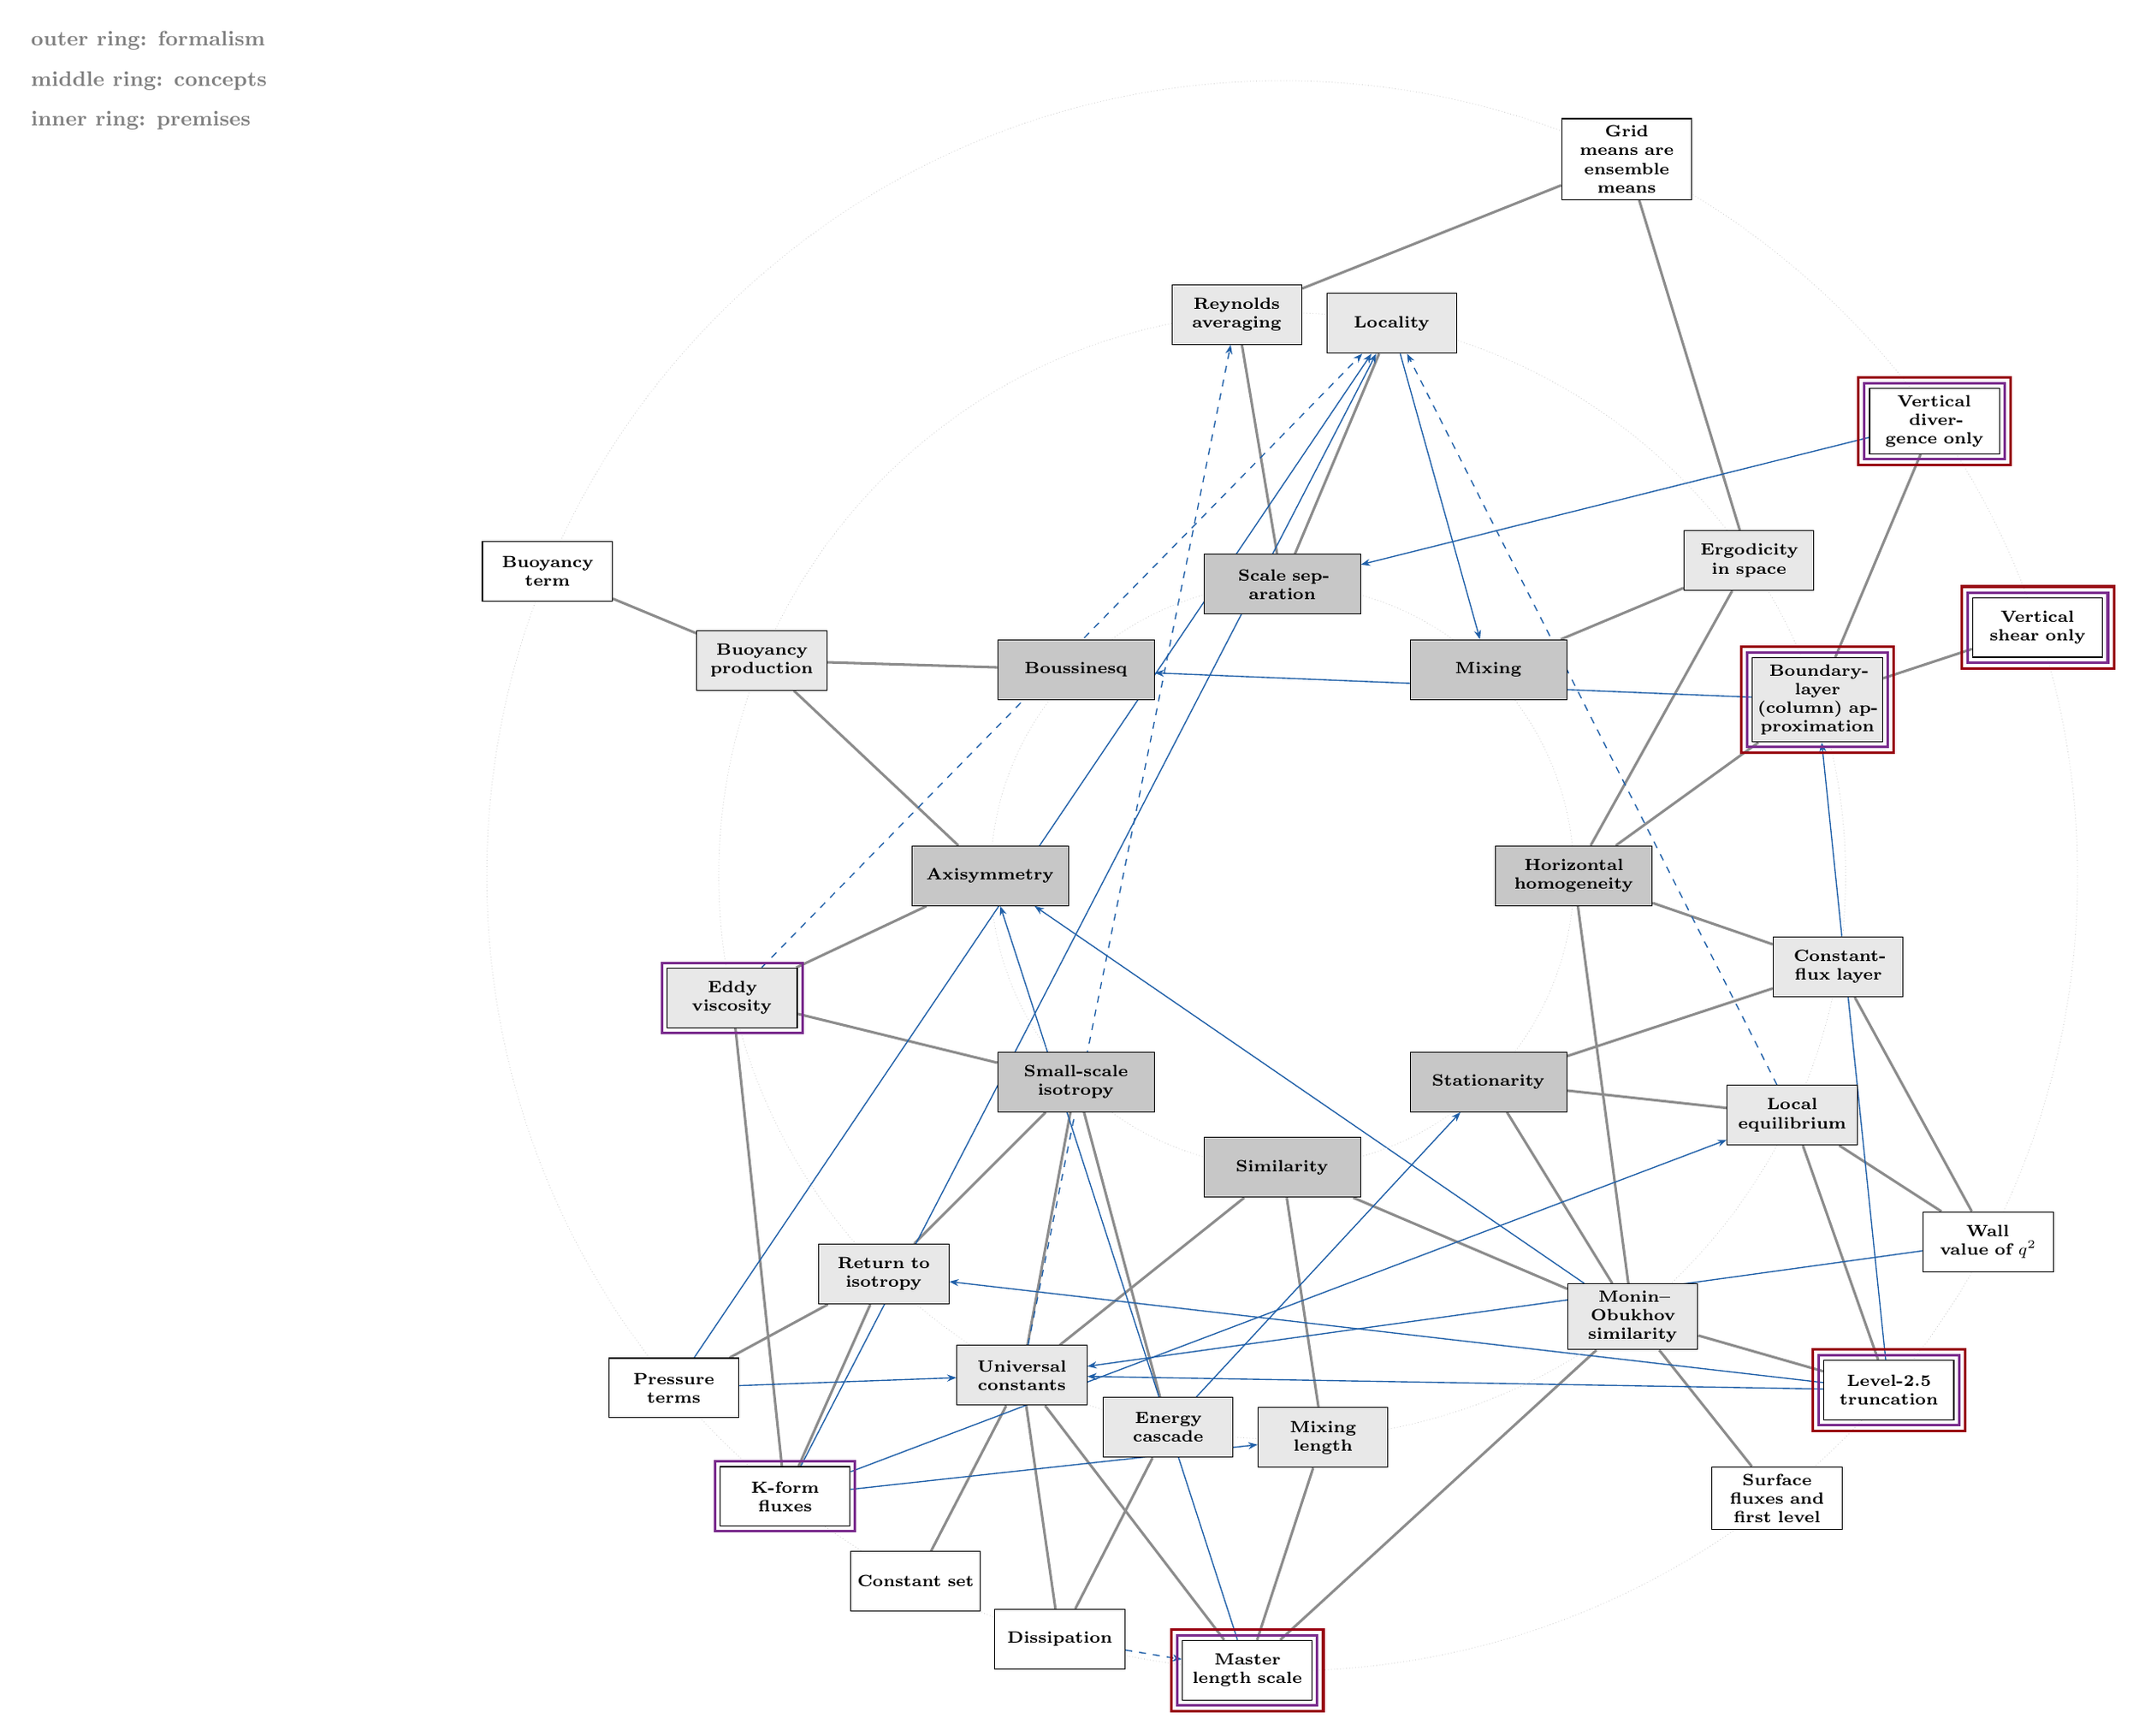
\begin{tikzpicture}[x=1cm, y=1cm]
\draw[ring] (0,0) circle (4.4);
\draw[ring] (0,0) circle (8.5);
\draw[ring] (0,0) circle (12.0);
\node[tier] at (90:5.15) {};
\node[tier] at (90:9.25) {};
\node[tier] at (90:12.75) {};
\node[nd, fill=black!22, text width=2.15cm] (n0) at (90.00:4.4) {\textbf{Scale separation}};
\node[nd, fill=black!22, text width=2.15cm] (n1) at (45.00:4.4) {\textbf{Mixing}};
\node[nd, fill=black!22, text width=2.15cm] (n2) at (0.00:4.4) {\textbf{Horizontal homogeneity}};
\node[nd, fill=black!22, text width=2.15cm] (n3) at (-45.00:4.4) {\textbf{Stationarity}};
\node[nd, fill=black!22, text width=2.15cm] (n4) at (-90.00:4.4) {\textbf{Similarity}};
\node[nd, fill=black!22, text width=2.15cm] (n5) at (-135.00:4.4) {\textbf{Small-scale isotropy}};
\node[nd, fill=black!22, text width=2.15cm] (n6) at (-180.00:4.4) {\textbf{Axisymmetry}};
\node[nd, fill=black!22, text width=2.15cm] (n7) at (-225.00:4.4) {\textbf{Boussinesq}};
\node[nd, fill=black!9, text width=1.75cm] (n8) at (78.78:8.5) {\textbf{Locality}};
\node[nd, fill=black!9, text width=1.75cm] (n9) at (94.62:8.5) {\textbf{Reynolds averaging}};
\node[nd, fill=black!9, text width=1.75cm] (n10) at (34.05:8.5) {\textbf{Ergodicity in space}};
\node[nd, fill=black!9, text width=1.75cm] (n11) at (18.21:8.5) {\textbf{Boundary-layer (column) approximation}};
\node[nd, fill=black!9, text width=1.75cm] (n12) at (350.70:8.5) {\textbf{Constant-flux layer}};
\node[nd, fill=black!9, text width=1.75cm] (n13) at (334.86:8.5) {\textbf{Local equilibrium}};
\node[nd, fill=black!9, text width=1.75cm] (n14) at (308.48:8.5) {\textbf{Monin--Obukhov similarity}};
\node[nd, fill=black!9, text width=1.75cm] (n15) at (274.16:8.5) {\textbf{Mixing length}};
\node[nd, fill=black!9, text width=1.75cm] (n16) at (242.48:8.5) {\textbf{Universal constants}};
\node[nd, fill=black!9, text width=1.75cm] (n17) at (258.32:8.5) {\textbf{Energy cascade}};
\node[nd, fill=black!9, text width=1.75cm] (n18) at (225.00:8.5) {\textbf{Return to isotropy}};
\node[nd, fill=black!9, text width=1.75cm] (n19) at (192.51:8.5) {\textbf{Eddy viscosity}};
\node[nd, fill=black!9, text width=1.75cm] (n20) at (157.50:8.5) {\textbf{Buoyancy production}};
\node[nd, fill=white, text width=1.75cm] (n21) at (64.33:12.0) {\textbf{Grid means are ensemble means}};
\node[nd, fill=white, text width=1.75cm] (n22) at (18.21:12.0) {\textbf{Vertical shear only}};
\node[nd, fill=white, text width=1.75cm] (n23) at (34.89:12.0) {\textbf{Vertical divergence only}};
\node[nd, fill=white, text width=1.75cm] (n24) at (332.60:12.0) {\textbf{Wall value of $\qsq$}};
\node[nd, fill=white, text width=1.75cm] (n25) at (319.70:12.0) {\textbf{Level-2.5 truncation}};
\node[nd, fill=white, text width=1.75cm] (n26) at (308.48:12.0) {\textbf{Surface fluxes and first level}};
\node[nd, fill=white, text width=1.75cm] (n27) at (267.48:12.0) {\textbf{Master length scale}};
\node[nd, fill=white, text width=1.75cm] (n28) at (242.54:12.0) {\textbf{Constant set}};
\node[nd, fill=white, text width=1.75cm] (n29) at (253.76:12.0) {\textbf{Dissipation}};
\node[nd, fill=white, text width=1.75cm] (n30) at (220.10:12.0) {\textbf{Pressure terms}};
\node[nd, fill=white, text width=1.75cm] (n31) at (231.32:12.0) {\textbf{K-form fluxes}};
\node[nd, fill=white, text width=1.75cm] (n32) at (157.50:12.0) {\textbf{Buoyancy term}};
\begin{scope}[on background layer]
\draw[contact] (n8) -- (n0);
\draw[contact] (n9) -- (n0);
\draw[contact] (n10) -- (n1);
\draw[contact] (n10) -- (n2);
\draw[contact] (n11) -- (n2);
\draw[contact] (n12) -- (n2);
\draw[contact] (n12) -- (n3);
\draw[contact] (n13) -- (n3);
\draw[contact] (n14) -- (n2);
\draw[contact] (n14) -- (n3);
\draw[contact] (n14) -- (n4);
\draw[contact] (n15) -- (n4);
\draw[contact] (n16) -- (n4);
\draw[contact] (n16) -- (n5);
\draw[contact] (n17) -- (n5);
\draw[contact] (n18) -- (n5);
\draw[contact] (n19) -- (n5);
\draw[contact] (n19) -- (n6);
\draw[contact] (n20) -- (n6);
\draw[contact] (n20) -- (n7);
\draw[contact] (n21) -- (n9);
\draw[contact] (n21) -- (n10);
\draw[contact] (n22) -- (n11);
\draw[contact] (n23) -- (n11);
\draw[contact] (n24) -- (n12);
\draw[contact] (n24) -- (n13);
\draw[contact] (n25) -- (n13);
\draw[contact] (n25) -- (n14);
\draw[contact] (n26) -- (n14);
\draw[contact] (n27) -- (n14);
\draw[contact] (n27) -- (n15);
\draw[contact] (n27) -- (n16);
\draw[contact] (n28) -- (n16);
\draw[contact] (n29) -- (n16);
\draw[contact] (n29) -- (n17);
\draw[contact] (n30) -- (n18);
\draw[contact] (n31) -- (n18);
\draw[contact] (n31) -- (n19);
\draw[contact] (n32) -- (n20);
\draw[lean] (n8) -- (n1);
\draw[lean] (n11) -- (n7);
\draw[lean] (n14) -- (n6);
\draw[lean] (n17) -- (n3);
\draw[leansame] (n13) -- (n8);
\draw[leansame] (n19) -- (n8);
\draw[leansame] (n16) -- (n9);
\draw[lean] (n23) -- (n0);
\draw[lean] (n24) -- (n16);
\draw[lean] (n25) -- (n18);
\draw[lean] (n25) -- (n16);
\draw[lean] (n25) -- (n11);
\draw[lean] (n27) -- (n6);
\draw[lean] (n30) -- (n8);
\draw[lean] (n30) -- (n16);
\draw[lean] (n31) -- (n8);
\draw[lean] (n31) -- (n15);
\draw[lean] (n31) -- (n13);
\draw[leansame] (n29) -- (n27);
\end{scope}
\draw[cFULL, line width=1.1pt] ($(n11.south west)+(-0.07,-0.07)$) rectangle ($(n11.north east)+(0.07,0.07)$);
\draw[cGXIX, line width=1.1pt] ($(n11.south west)+(-0.16,-0.16)$) rectangle ($(n11.north east)+(0.16,0.16)$);
\draw[cFULL, line width=1.1pt] ($(n22.south west)+(-0.07,-0.07)$) rectangle ($(n22.north east)+(0.07,0.07)$);
\draw[cGXIX, line width=1.1pt] ($(n22.south west)+(-0.16,-0.16)$) rectangle ($(n22.north east)+(0.16,0.16)$);
\draw[cFULL, line width=1.1pt] ($(n23.south west)+(-0.07,-0.07)$) rectangle ($(n23.north east)+(0.07,0.07)$);
\draw[cGXIX, line width=1.1pt] ($(n23.south west)+(-0.16,-0.16)$) rectangle ($(n23.north east)+(0.16,0.16)$);
\draw[cFULL, line width=1.1pt] ($(n25.south west)+(-0.07,-0.07)$) rectangle ($(n25.north east)+(0.07,0.07)$);
\draw[cGXIX, line width=1.1pt] ($(n25.south west)+(-0.16,-0.16)$) rectangle ($(n25.north east)+(0.16,0.16)$);
\draw[cFULL, line width=1.1pt] ($(n27.south west)+(-0.07,-0.07)$) rectangle ($(n27.north east)+(0.07,0.07)$);
\draw[cGXIX, line width=1.1pt] ($(n27.south west)+(-0.16,-0.16)$) rectangle ($(n27.north east)+(0.16,0.16)$);
\draw[cFULL, line width=1.1pt] ($(n19.south west)+(-0.07,-0.07)$) rectangle ($(n19.north east)+(0.07,0.07)$);
\draw[cFULL, line width=1.1pt] ($(n31.south west)+(-0.07,-0.07)$) rectangle ($(n31.north east)+(0.07,0.07)$);
\node[tier, anchor=west] at (-19.0, 12.6) {outer ring: formalism};
\node[tier, anchor=west] at (-19.0, 12.0) {middle ring: concepts};
\node[tier, anchor=west] at (-19.0, 11.4) {inner ring: premises};
\end{tikzpicture}
\end{center}
\end{document}
